\documentclass{beamer}

% Direct LaTeX to look inside the "theme" subfolder for .sty files
\makeatletter
\def\input@path{{./theme/}}
\makeatother

\usetheme{metropolis}

\usepackage{tikz}

\title{Covering Families for Complete Bipartite Graphs with DP-Coloring}
\date{\today}
\author{Illia Siutkin}
\institute{Lake Forest College}
\begin{document}
  \maketitle
  
  \section{Introduction to DP-Coloring}
  
  \frame{{Graph Coloring}
  
  \vspace{0.3cm}
  Allocation of colors to the vertices. In a proper coloring, adjacent vertices receive different colors.
  \vspace{0.5cm}

  \centering

  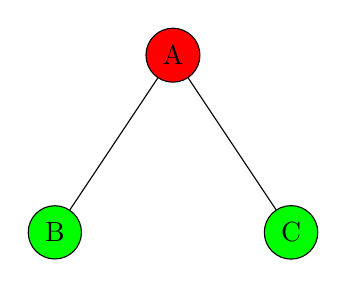
\begin{tikzpicture}[scale=1.5]
        % vertices
        \node[circle, draw, fill = red] (A) at (1,1.5) {A};
        \node[circle, draw, fill = green] (B) at (0,0) {B};
        \node[circle, draw, fill = green] (C) at (2,0) {C};
    
        % edges
        \draw (A) -- (B);
        \draw (A) -- (C);
    \end{tikzpicture}

}
  
\end{document}